\documentclass{article}
\usepackage[a4paper, margin=1in]{geometry}  % Set uniform 1-inch margins
\usepackage{tikz}
\title{Lab Final}
\author{Sumaiya Tabassum}
\begin{document}

	\begin{center}
		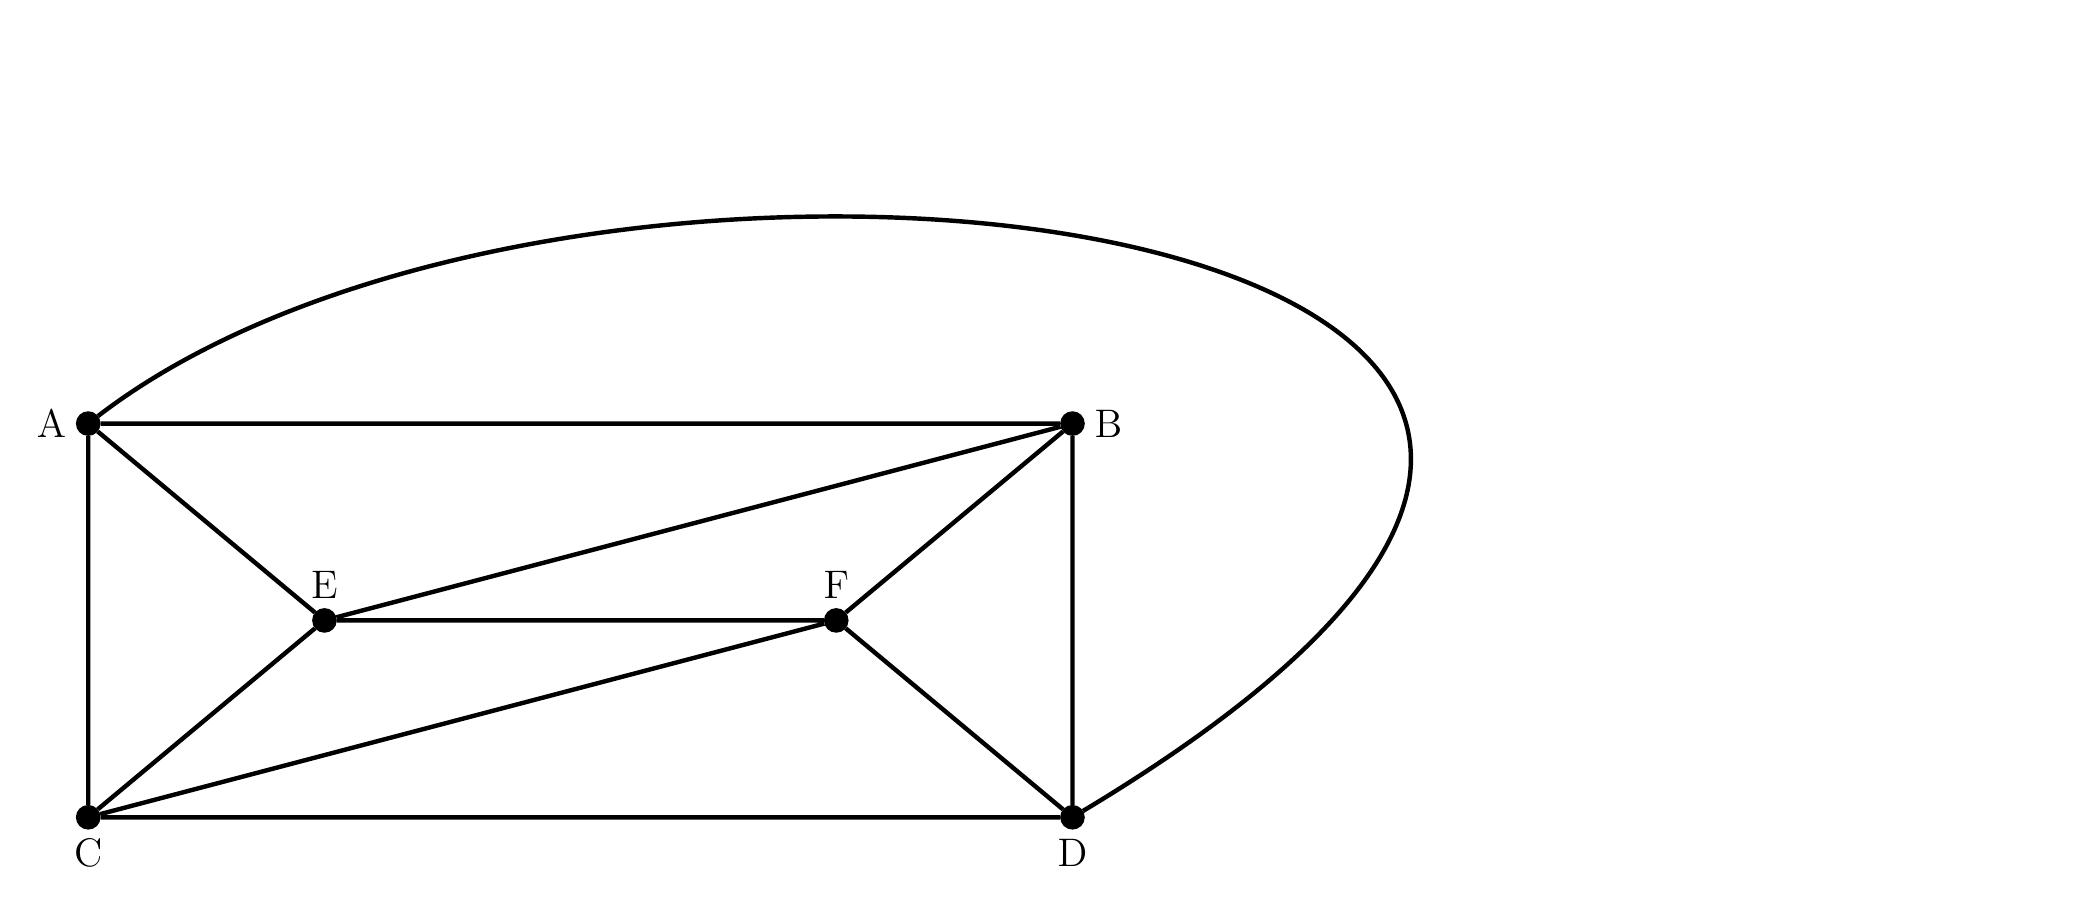
\begin{tikzpicture}[scale=5]
			\node(C) at (0,0)[circle,fill=black,text=white,inner sep=3pt,label=below:\Large C,draw]{};
			\node(A) at (0,1)[circle,fill=black,text=white,inner sep=3pt,label=left:\Large A,draw]{};
			\node(D) at (2.5,0)[circle,fill=black,text=white,inner sep=3pt,label=below:\Large D,draw]{};
			\node(B) at (2.5,1)[circle,fill=black,text=white,inner sep=3pt,label=right:\Large B,draw]{};
			
			\node(E) at (0.6,0.5)[circle,fill=black,text=white,inner sep=3pt,label=above:\Large E,draw]{};
			\node(F) at (1.9,0.5)[circle,fill=black,text=white,inner sep=3pt,label=above:\Large F,draw]{};
			
			\draw[-,ultra thick] (A) to (B) to (D) to (C) to (A) to (E) to (C) to (F) to (E) to (B) to (F) to (D);
			\draw[ultra thick] (A) ..controls (1.3,2) and (5,1.5) ..(D);
		\end{tikzpicture}
	\end{center}

\end{document}